%%%%%%%%%%%%%%%%%%%%%%%%%%%%%%%%%%%%%%%%%%%%%%%%%%%%%%%%%%%%%%%%%%%%%%%%%%%%%%%%%%
\begin{frame}[fragile]\frametitle{}

\begin{center}
{\Large Linguistics}
\end{center}
\end{frame}

 %%%%%%%%%%%%%%%%%%%%%%%%%%%%%%%%%%%%%%%%%%%%%%%%%%%%%%%%%%%%%%%%%%%%%%%%%%%%%%%%%%
\begin{frame}[fragile]
  \frametitle{Introduction}
  \begin{itemize}
  \item Obviously, this is not about NLP or Linguistics in a classical sense, so very superficial, 
  \item We just want to discuss how to make progress in natural language understanding
  \item 
Introduce basic linguistics concepts. 
  \item 
Basic terminology 
  \item 
Discuss the levels of analysis used in NLP 
  \item 
Problems associated with each level.

  	  \end{itemize}
 \end{frame} 
 
  
%%%%%%%%%%%%%%%%%%%%%%%%%%%%%%%%%%%%%%%%%%%%%%%%%%%%%%%%%%%%%%%%%%%%%%%%%%%%%%%%%%
\begin{frame}[fragile]
  \frametitle{Levels of Analysis}
  \begin{center}
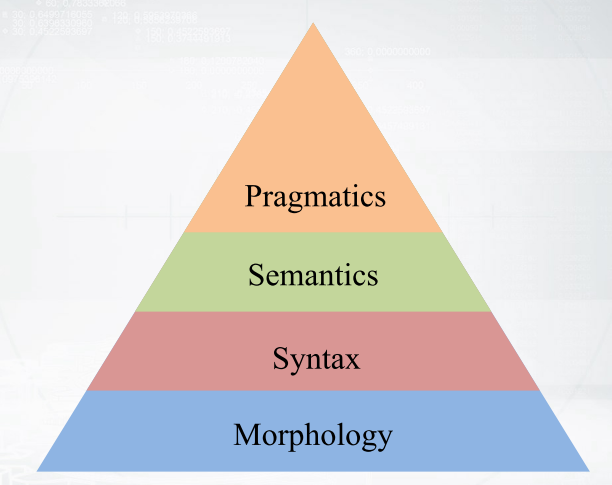
\includegraphics[width=0.7\linewidth,keepaspectratio]{lingpyr}
\end{center}



(Ref: https://www.coursera.org/learn/language-processing/lecture/j8kee/main-approaches-in-nlp)
 \end{frame}

 
 %%%%%%%%%%%%%%%%%%%%%%%%%%%%%%%%%%%%%%%%%%%%%%%%%%%%%%%%%%%%%%%%%%%%%%%%%%%%%%%%%%
\begin{frame}[fragile]
  \frametitle{Levels of Analysis}
  In traditional linguistics people talk about several levels of analysis, or types of linguistics knowledge. 

  \begin{itemize}
  \item Morphology:
How words are constructed
 \item Syntax:
Structural relation between words
 \item Semantics :
The meaning of words and of combinations fo words
 \item Pragmatics: 
How a sentence is used? What’s its purpose
 \item Discourse (sometimes distinguished as a subfield of Pragmatics):
Relationships between sentences; global context. 
  	  \end{itemize}
 \end{frame} 
 



 %%%%%%%%%%%%%%%%%%%%%%%%%%%%%%%%%%%%%%%%%%%%%%%%%%%%%%%%%%%%%%%%%%%%%%%%%%%%%%%%%%
\begin{frame}[fragile]
  \frametitle{Morphology}
  \begin{itemize}
  \item About different forms of words. 
  \item In traditional linguistics morphology analyses how words are formed, what is their origin, how does their form change depending on the context
  \item For example, we care about part of speech text, we care about different cases and genders and tenses. 
  \item So this is everything that goes just for single words in the sentence.
  	  \end{itemize}
 \end{frame} 
 


 %%%%%%%%%%%%%%%%%%%%%%%%%%%%%%%%%%%%%%%%%%%%%%%%%%%%%%%%%%%%%%%%%%%%%%%%%%%%%%%%%%
\begin{frame}[fragile]
  \frametitle{Morphology}
  In NLP you’ll mostly deal with
  \begin{itemize}
  \item prefixes/suffixes
  \item singularization/pluralization
  \item gender detection
  \item word inflection
  \item lemmatization (the base form of a word).
  \item Spell-checking
  	  \end{itemize}
	  
In morphology, most of the operations are at a word level, where a word is viewed as a sequence of characters.	  
 \end{frame} 
 
   %%%%%%%%%%%%%%%%%%%%%%%%%%%%%%%%%%%%%%%%%%%%%%%%%%%%%%%%%%%%%%%%%%%%%%%%%%%%%%%%%%
\begin{frame}[fragile]
  \frametitle{Morphology}
  \begin{itemize}
  \item The simple cases are:
                         kick, kicks, kicked, kicking
  \item TBut other cases may be:
                          sit, sits, sat, sitting
 Not just as simple as adding and deleting certain endings, as in:
 
                         gorge, gorgeous    
						 
                         good, goods    
						 
                         arm, army
  \item TThis might be very different in other languages
  	  \end{itemize}
 \end{frame} 
 
 
 %%%%%%%%%%%%%%%%%%%%%%%%%%%%%%%%%%%%%%%%%%%%%%%%%%%%%%%%%%%%%%%%%%%%%%%%%%%%%%%%%%
\begin{frame}[fragile]
  \frametitle{Syntax}
  \begin{itemize}
  \item Syntactical analysis, will be about different relations between words in the sentence.
  \item Syntax cares about what proper word constructions are. Determining the underlying structure of a sentence or building valid sentences is what syntax is all about. 
  \item In a way, syntax is what we usually refer to as grammar.
  \item For example, we can know that there are some objects and subjects and so on. 
  % \item Syntax concerns the way in which words can be combined together to form
% (grammatical) sentences; 
% \item eg. ``revolutionary new ideas appear infrequently'' is
% grammatical in English, 
% \item ``colourless green ideas sleep furiously'' is grammatical
% but nonsensical, 
% \item whilst ``*ideas green furiously colourless sleep'' is ungrammatical too. 
% \item Note: Linguists use asterisks to indicate ‘ungrammaticality’, or illegality
% given the rules of a language.
  	  \end{itemize}
 \end{frame} 
 
  %%%%%%%%%%%%%%%%%%%%%%%%%%%%%%%%%%%%%%%%%%%%%%%%%%%%%%%%%%%%%%%%%%%%%%%%%%%%%%%%%%
\begin{frame}[fragile]
  \frametitle{Syntax}
  Syntax is probably the most researched branch of computational linguistics. Here are only a few of the tasks related to Syntax:
  \begin{itemize}
  \item Part-of-speech tagging (assigning tags to words: Noun/Verb/Adjective/Adverb/Pronoun/Preposition Conjunction etc )
\item Building Syntax Trees
\item Building Dependency Trees
  	  \end{itemize}
	  Syntax usually works on sentences, where a sentence is a sequence of words.
 \end{frame} 
 
 
    %%%%%%%%%%%%%%%%%%%%%%%%%%%%%%%%%%%%%%%%%%%%%%%%%%%%%%%%%%%%%%%%%%%%%%%%%%%%%%%%%%
\begin{frame}[fragile]
  \frametitle{Syntax}
  \begin{itemize}
  \item The main issues here are structural ambiguities, as in:
                        I saw the Grand Canyon flying to New York.
						
or 

                        Time flies like an arrow. 
						
  \item The sentence can be interpreted as a 
  \begin{itemize}
  \item Metaphor: time passes quickly, but also 
  \item Declaratively: Insects have an affinity for arrows 
  \item Imperative: measure the time of the insects. 
    	  \end{itemize}

  \item Key issue: Often syntax doesn't tell us much about meaning. 
  
                          Plastic cat food can cover

  	  \end{itemize}
 \end{frame} 
 
  %%%%%%%%%%%%%%%%%%%%%%%%%%%%%%%%%%%%%%%%%%%%%%%%%%%%%%%%%%%%%%%%%%%%%%%%%%%%%%%%%%
\begin{frame}[fragile]
  \frametitle{Semantics}
  \begin{itemize}
  \item  Once we know some Syntactical structures, next would be about semantics. 
  \item So semantics is about the meaning. 
  \item Going from just some symbols to some meanings.
  \item Because the meaning of a sentence is usually a productive combination of
the meaning of its words, syntactic information is important for interpretation
– it helps us work out what goes with what – but other information, such as
punctuation or intonation, pronoun reference, etc, can also play a crucial part.
  	  \end{itemize}
 \end{frame} 
 
   %%%%%%%%%%%%%%%%%%%%%%%%%%%%%%%%%%%%%%%%%%%%%%%%%%%%%%%%%%%%%%%%%%%%%%%%%%%%%%%%%%
\begin{frame}[fragile]
  \frametitle{Semantics}
  Here are some known Semantics related problems:
  \begin{itemize}
  \item  Named Entity Extraction
  \item  Relation Extraction
  % \item  Semantic Role Labelling
  \item  Word Sense Disambiguation
  	  \end{itemize}
Semantics usually works on sentences, where a sentence is a sequence of words usually with some added semantics (like sense, role) attached.	  
 \end{frame} 
 
   %%%%%%%%%%%%%%%%%%%%%%%%%%%%%%%%%%%%%%%%%%%%%%%%%%%%%%%%%%%%%%%%%%%%%%%%%%%%%%%%%%
\begin{frame}[fragile]
  \frametitle{Semantics}
  Some key issue here: 

  
  \begin{itemize}
  \item  Lexical ambiguities:

                  I walked to the bank      {of the river / to get money}.

                  The bug in the room   {was probably planted by spies /   
                                                        flew out the window}. 
  \item  Compositionality: The meaning of phrases/sentences as a function of the meaning of words in them.

  	  \end{itemize}
 \end{frame} 
 
   %%%%%%%%%%%%%%%%%%%%%%%%%%%%%%%%%%%%%%%%%%%%%%%%%%%%%%%%%%%%%%%%%%%%%%%%%%%%%%%%%%
\begin{frame}[fragile]
  \frametitle{Pragmatics/Discourse}
  \begin{itemize}
  \item Pragmatics would be the highest level of this abstraction.
  \item   Pragmatics analyses the text as a whole. It’s about determining underlying narrative threads, topics, references.
  \item Pragmatics is about the use of language in context, where context includes
both the linguistic and situational context of an utterance; eg. if I say ``Draw
the curtains'' in a situation where the curtains are open this is likely to be a
command to someone present to shut the curtains (and vice versa if they are
closed).
  	  \end{itemize}
 \end{frame} 
 
  
    %%%%%%%%%%%%%%%%%%%%%%%%%%%%%%%%%%%%%%%%%%%%%%%%%%%%%%%%%%%%%%%%%%%%%%%%%%%%%%%%%%
\begin{frame}[fragile]
  \frametitle{Pragmatics/Discourse}
  \begin{itemize}
  \item Pragmatics:  How a sentence is used; its purpose. 
\item Discourse:  Relations between sentences; global context.

  	  \end{itemize}
 \end{frame} 
 
    %%%%%%%%%%%%%%%%%%%%%%%%%%%%%%%%%%%%%%%%%%%%%%%%%%%%%%%%%%%%%%%%%%%%%%%%%%%%%%%%%%
\begin{frame}[fragile]
  \frametitle{Pragmatics/Discourse}
  Some Pragmatics tasks are:
  \begin{itemize}
  \item Co-reference / Anaphora resolution (find out what word refers what. Example: John is fine. He[John]‘s in no danger.)
  \item Topic segmentation
  % \item Lexical chains
  \item Summarization
  	  \end{itemize}
 \end{frame} 
 

 
 
 % %%%%%%%%%%%%%%%%%%%%%%%%%%%%%%%%%%%%%%%%%%%%%%%%%%%%%%%%%%%%%%%%%%%%%%%%%%%%%%%%%%
% \begin{frame}[fragile]
  % \frametitle{Linguistics Tools}
  % \begin{itemize}
  % \item Grammar: Study of language structure
  % \item Semantics: Study of meaning
  	  % \end{itemize}
 % \end{frame}

% %%%%%%%%%%%%%%%%%%%%%%%%%%%%%%%%%%%%%%%%%%%%%%%%%%%%%%%%%%%%%%%%%%%%%%%%%%%%%%%%%%
% \begin{frame}[fragile]
  % \frametitle{Linguistics Essentials}
  % \begin{itemize}

    % \item For Morphological and Syntactical processing: Nltk, Stanford parser
        % \item For Semantics: topic modeling, word2vec: Gensim, Mallet
  	  % \end{itemize}
 % \end{frame}


% %%%%%%%%%%%%%%%%%%%%%%%%%%%%%%%%%%%%%%%%%%%%%%%%%%%%%%%%%%%%%%%%%%%%%%%%%%%%%%%%%%
% \begin{frame}[fragile]
  % \frametitle{Linguistics Essentials}
% Grammar:
	    % \begin{itemize}
	  % \item Phonology: Study of sound systems
	  % \item Morphology (the formation and composition of words)
	  % \item Syntax (the rules that determine how words combine into sentences) 

	  % \end{itemize}
% \end{frame}

% %%%%%%%%%%%%%%%%%%%%%%%%%%%%%%%%%%%%%%%%%%%%%%%%%%%%%%%%%%%%%%%%%%%%%%%%%%%%%%%%%%
% \begin{frame}[fragile]
  % \frametitle{Linguistics Essentials}
 % Semantics:
	    % \begin{itemize}
	  % \item The study of the meaning of words (lexical semantics) and fixed word combinations (phraseology), 
	  % \item How these combine to form the meanings of sentences 
	  % \end{itemize}  
% \end{frame}


%%%%%%%%%%%%%%%%%%%%%%%%%%%%%%%%%%%%%%%%%%%%%%%%%%%%%%%%%%%%%%%%%%%%%%%%%%%%%%%%%%%
%\begin{frame}[fragile]
%  \frametitle{Linguistics sub-fields}
%  \begin{itemize}
%  \item Discourse analysis 
%	    \begin{itemize}
%	  \item Concerned with the structure of texts and conversations
%	  \end{itemize}
%  \item Pragmatics:
%	    \begin{itemize}
%	  \item Concerned with how meaning is transmitted based on a combination of linguistic competence, non-linguistic knowledge, and the context of the speech act.
%	  \end{itemize}  
%  \end{itemize}
%\end{frame}

%%%%%%%%%%%%%%%%%%%%%%%%%%%%%%%%%%%%%%%%%%%%%%%%%%%%%%%%%%%%%%%%%%%%%%%%%%%%%%%%%%
\begin{frame}[fragile]\frametitle{}

\begin{center}
{\Large Linguistics, in details (Adv)}
\end{center}
\end{frame}


%%%%%%%%%%%%%%%%%%%%%%%%%%%%%%%%%%%%%%%%%%%%%%%%%%%%%%%%%%%%%%%%%%%%%%%%%%%%%%%%%%
\begin{frame}[fragile]
  \frametitle{Morphology}
  \begin{itemize}
  \item Morphology is the study of the internal structure of words, of the way words are built up from smaller meaning units.
  \item Morpheme: The smallest meaningful unit in the grammar.
  \end{itemize}
\end{frame}

%%%%%%%%%%%%%%%%%%%%%%%%%%%%%%%%%%%%%%%%%%%%%%%%%%%%%%%%%%%%%%%%%%%%%%%%%%%%%%%%%%
\begin{frame}[fragile]
  \frametitle{Morphology}
Two classes of morphemes
    \begin{itemize}
  \item Stems: ``main'' morpheme of the word, supplying the main meaning (i.e. establish in the example below)
  \item Affixes: add additional meaning
    \begin{itemize}
  \item Prefixes: Antidisestablishmentarianism
  \item Suffixes: Antidisestablishmentarianism
  \item Infixes: hingi (borrow) - humingi (borrower) in Tagalog
  \item Circumfixes: sagen (say) - gesagt (said) in German
    \end{itemize}
  \end{itemize}
\end{frame}

%%%%%%%%%%%%%%%%%%%%%%%%%%%%%%%%%%%%%%%%%%%%%%%%%%%%%%%%%%%%%%%%%%%%%%%%%%%%%%%%%%
\begin{frame}[fragile]
  \frametitle{Morphology: examples}
Unladylike
    \begin{itemize}
  \item The word unladylike consists of three morphemes and four syllables. 
  \item Morpheme breaks:
      \begin{itemize}
  \item un- 'not' 
  \item lady '(well behaved) female adult human' 
  \item -like 'having the characteristics of' 
      \end{itemize}
  \item None of these morphemes can be broken up any more without losing all sense of meaning. Lady cannot be broken up into "la" and "dy," even though "la" and "dy" are separate syllables. Note that each syllable has no meaning on its own. 
    \end{itemize}
\end{frame}

%%%%%%%%%%%%%%%%%%%%%%%%%%%%%%%%%%%%%%%%%%%%%%%%%%%%%%%%%%%%%%%%%%%%%%%%%%%%%%%%%%
\begin{frame}[fragile]
  \frametitle{Types of morphological processes}
  Inflection:
  \begin{itemize}
  \item Systematic modification of a root form by means  of prefixes and suffixes to indicate grammatical distinctions like singular and plural. 
  \item Stems: also called lemma, base form, root, lexeme
  \item Doesn't change the word class
  \item New grammatical role
  \item Usually produces a predictable, non idiosyncratic change of meaning. 
  \item run : runs | running | ran
  \item hope+ing : hoping;	hop : hopping

  \end{itemize}
\end{frame}

%%%%%%%%%%%%%%%%%%%%%%%%%%%%%%%%%%%%%%%%%%%%%%%%%%%%%%%%%%%%%%%%%%%%%%%%%%%%%%%%%%
\begin{frame}[fragile]
  \frametitle{Types of morphological processes}
  Derivation:
  \begin{itemize}
  \item Ex: compute :  computer : computerization
  \item Less systematic that inflection
  \item It can involve a change of meaning
  \item Wide: Widely
  \item Suffix en transforms adjective into verbs: Weak : weaken, soft: soften
  \item Suffix able transforms verbs into adjective: Understand : Understandable
  \item Suffix er transforms verbs into nouns (nominalization): teach : teacher
  \item Difficult cases: building : from which sense of ``build''?
  \end{itemize}
\end{frame}

%%%%%%%%%%%%%%%%%%%%%%%%%%%%%%%%%%%%%%%%%%%%%%%%%%%%%%%%%%%%%%%%%%%%%%%%%%%%%%%%%%
\begin{frame}[fragile]
  \frametitle{Types of morphological processes}
  Compounding:
  \begin{itemize}
  \item Merging of two or more words into a new word
  \item Downmarket, (to) overtake

  \end{itemize}
\end{frame}


% %%%%%%%%%%%%%%%%%%%%%%%%%%%%%%%%%%%%%%%%%%%%%%%%%%%%%%%%%%%%%%%%%%%%%%%%%%%%%%%%%%
% \begin{frame}[fragile]\frametitle{}

% \begin{center}
% {\Large Syntax/Grammar, in details}
% \end{center}
% \end{frame}



%%%%%%%%%%%%%%%%%%%%%%%%%%%%%%%%%%%%%%%%%%%%%%%%%%%%%%%%%%%%%%%%%%%%%%%%%%%%%%%%%%
\begin{frame}[fragile]
  \frametitle{Grammar: Words}
  \begin{itemize}
  \item Words of a language are grouped into classes to reflect similar syntactic behaviors
  \item Syntactical or grammatical categories (aka part-of-speech)
       \begin{itemize}
	  \item Nouns (people, animal, concepts)
	  \item Verbs (actions, states)
	  \item Adjectives
	  \item Prepositions
	  \item Conjunction
	  \item Interjections
	  \end{itemize}
  \end{itemize}
\end{frame}

%%%%%%%%%%%%%%%%%%%%%%%%%%%%%%%%%%%%%%%%%%%%%%%%%%%%%%%%%%%%%%%%%%%%%%%%%%%%%%%%%%
\begin{frame}[fragile]
  \frametitle{Grammar}
  \begin{center}
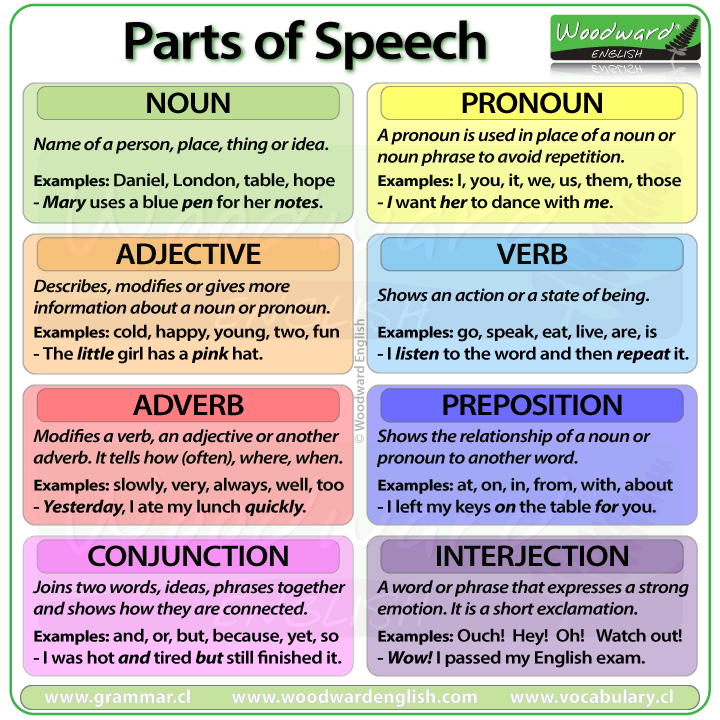
\includegraphics[width=0.6\linewidth,keepaspectratio]{pos}
\end{center}
\end{frame}

%%%%%%%%%%%%%%%%%%%%%%%%%%%%%%%%%%%%%%%%%%%%%%%%%%%%%%%%%%%%%%%%%%%%%%%%%%%%%%%%%%%
%\begin{frame}[fragile]
%  \frametitle{Grammar: words}
%       \begin{itemize}
%	  \item Nouns (people, animal, concepts): नाम, संज्ञा
%	  \item Pronoun (in place of nouns, he she, they): सर्वनाम
%	  \item Verbs (actions, states):क्रियापद
%	  \item Adjectives(more about nouns): विशेषण
%	  \item Adverb(more about verb): क्रियाविशेषण
%	  \item Prepositions (relationship, inside, outside,): संबंधशोधक, शब्दयोगी अव्यय
%	  \item Conjunctions (joiners): समुच्चयबोधक, योजक, उभयान्वयी अव्यय
%	  \item Interjections (surprise, oh, wow): विस्मयबोधक, केवलप्रयोगी अव्यय
%	  \end{itemize}
%\end{frame}


%%%%%%%%%%%%%%%%%%%%%%%%%%%%%%%%%%%%%%%%%%%%%%%%%%%%%%%%%%%%%%%%%%%%%%%%%%%%%%%%%%
\begin{frame}[fragile]
  \frametitle{Grammar: English + Indic}
       \begin{itemize}
	  \item Nouns (people, animal, concepts):$naam, sadnya$
	  \item Pronoun (in place of nouns, he she, they): $sarv\_  naam$
	  \item Verbs (actions, states): $kriyapad$
	  \item Adjectives(more about nouns): $visheshan$
	  \item Adverb(more about verb): $kriya\_ visheshan$
	  \item Prepositions (relationship, inside, outside,): $sambandh shodhak shabdayogi \_ avyay$
	  \item Conjunctions (joiners): $samuchchay bodhak, ubhayanvayi \_ avyay$
	  \item Interjections (surprise, oh, wow): $vismay bodhak, kevalprayogi\_ avyay$
	  	  \end{itemize}
\end{frame}


%%%%%%%%%%%%%%%%%%%%%%%%%%%%%%%%%%%%%%%%%%%%%%%%%%%%%%%%%%%%%%%%%%%%%%%%%%%%%%%%%%
\begin{frame}[fragile]
  \frametitle{Grammar: Expand-ability}
  \begin{itemize}
  \item Open or lexical categories (nouns, verbs, adjective):
	    \begin{itemize}
	  \item Large number of members, new words are commonly added
	  \end{itemize}  
\item Closed or functional categories (prepositions, determiners)
	    \begin{itemize}
	  \item Few members, clear grammatical use
	  \end{itemize}  
  \end{itemize}
\end{frame}

%%%%%%%%%%%%%%%%%%%%%%%%%%%%%%%%%%%%%%%%%%%%%%%%%%%%%%%%%%%%%%%%%%%%%%%%%%%%%%%%%%
\begin{frame}[fragile]
  \frametitle{Grammar: Morphology}
  Word categories are related by morphological processes
  \begin{itemize}
  \item `s' for plural nouns
  \item `ed' for verbs' past forms
  \item More important for some languages
  \item Finnish verbs have 10,000 forms
  \item Indian languages?
  \end{itemize}
\end{frame}

%%%%%%%%%%%%%%%%%%%%%%%%%%%%%%%%%%%%%%%%%%%%%%%%%%%%%%%%%%%%%%%%%%%%%%%%%%%%%%%%%%
\begin{frame}[fragile]
  \frametitle{Indian Grammar}
  \begin{center}
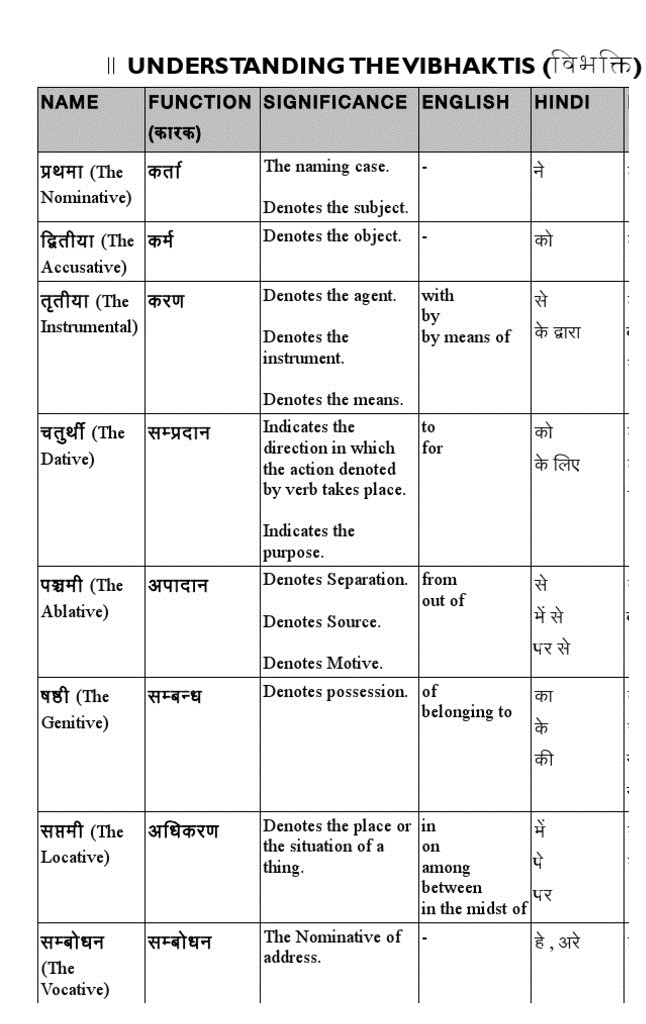
\includegraphics[width=0.4\linewidth,keepaspectratio]{vibhakti}
\end{center}
\end{frame}

%%%%%%%%%%%%%%%%%%%%%%%%%%%%%%%%%%%%%%%%%%%%%%%%%%%%%%%%%%%%%%%%%%%%%%%%%%%%%%%%%%
\begin{frame}[fragile]
  \frametitle{Grammatical categories: Nouns}
  \begin{itemize}
  \item Nouns typically refer to entities in the world like people, animals, things, ideas.. 
  \item Type of inflections
  \begin{itemize}
  \item Number 
  \item Gender 
  \item Case (nominative, genitive, accusative, dative)
  \end{itemize}
  \item Pronouns: variables to refer to an entity previously mentioned
  \end{itemize}
\end{frame}


%%%%%%%%%%%%%%%%%%%%%%%%%%%%%%%%%%%%%%%%%%%%%%%%%%%%%%%%%%%%%%%%%%%%%%%%%%%%%%%%%%
\begin{frame}[fragile]
  \frametitle{Grammatical categories: Verbs}
  \begin{itemize}
  \item Usually denote an action (bring, read), an occurrence (decompose, glitter), or a state of being (exist, stand). 
  \item Depending on the language, a verb may vary in form according to many factors, possibly including its tense, aspect, mood and voice. 
  \item It may also agree with the person, gender, and/or number of some of its arguments (subject, object, etc.) 
  \end{itemize}
\end{frame}

%%%%%%%%%%%%%%%%%%%%%%%%%%%%%%%%%%%%%%%%%%%%%%%%%%%%%%%%%%%%%%%%%%%%%%%%%%%%%%%%%%
\begin{frame}[fragile]
  \frametitle{Grammatical categories: Other}
  \begin{itemize}
  \item Adverbs: fast, slow
  \item Prepositions : in, on, over, at
  \item Coordinating Conjunctions are for linking two sentences: $and, or, but$, e.g. She bought $or$ leased the car
  \item Subordinating Conjunctions make one clause dependent (or ``subordinate'') upon the other: $that, because, if$, e.g.  She said $that$ she would lease a car
  \end{itemize}
\end{frame}


%%%%%%%%%%%%%%%%%%%%%%%%%%%%%%%%%%%%%%%%%%%%%%%%%%%%%%%%%%%%%%%%%%%%%%%%%%%%%%%%%%
\begin{frame}[fragile]
  \frametitle{Phrase structure}
  \begin{itemize}
  \item Words are organized in phrases
  \item Phrases: grouping of words that are clumped as a unit
  \item Syntax: study of the regularities and constraints of word order and phrase structure
  \end{itemize}
\end{frame}


%%%%%%%%%%%%%%%%%%%%%%%%%%%%%%%%%%%%%%%%%%%%%%%%%%%%%%%%%%%%%%%%%%%%%%%%%%%%%%%%%%
\begin{frame}[fragile]
  \frametitle{Syntactic Parsing}
  \begin{itemize}
  \item  The cat sat on the mat.
  
Det Noun Verb Prep Det Noun
  \item Time flies like an arrow.
  
Noun  Verb     Prep Det Noun
  \item Fruit flies like a banana.
  
Noun  Noun    Verb Det Noun
  \end{itemize}
\end{frame}

  
 

%%%%%%%%%%%%%%%%%%%%%%%%%%%%%%%%%%%%%%%%%%%%%%%%%%%%%%%%%%%%%%%%%%%%%%%%%%%%%%%%%%
\begin{frame}[fragile]
  \frametitle{Major phrase types}
  \begin{itemize}
  \item Sentence (S) (whole grammatical unit). Normally rewrites as a subject noun phrase and a verb phrase
  \item Noun phrase (NP): phrase whose head is a noun or a pronoun, optionally accompanied by a set of modifiers 
  \item   For example, ''Put the bread on the table'' needs ''on the table'' to make it complete. You cannot merely put something, you need to put it somewhere. In this context, the phrase ''on the table'' is a complement. 
  \item By contrast, ''The bread on the table is fresh.'' does not require ''on the table'' to be complete, so here, the phrase ''on the table'' is a modifier. A modifier, unlike a complement, is an optional element of a sentence. 
  \end{itemize}
\end{frame}

%%%%%%%%%%%%%%%%%%%%%%%%%%%%%%%%%%%%%%%%%%%%%%%%%%%%%%%%%%%%%%%%%%%%%%%%%%%%%%%%%%
\begin{frame}[fragile]
  \frametitle{Major phrase types}
  \begin{itemize}
  \item Prepositional phrases (PP): Headed by  a preposition and containing a NP: She is [on the computer]; They walked [to their school] 
  \item Verb phrases (VP): Phrase whose head is a verb:
    \begin{itemize}
  \item ``Getting to school on time'' was a struggle
  \item He ``was trying to keep his temper''
  \item That woman ``quickly showed me the way to hide''
  \end{itemize}
  \end{itemize}
\end{frame}



%%%%%%%%%%%%%%%%%%%%%%%%%%%%%%%%%%%%%%%%%%%%%%%%%%%%%%%%%%%%%%%%%%%%%%%%%%%%%%%%%%
\begin{frame}[fragile]
  \frametitle{Parses}
  \begin{center}
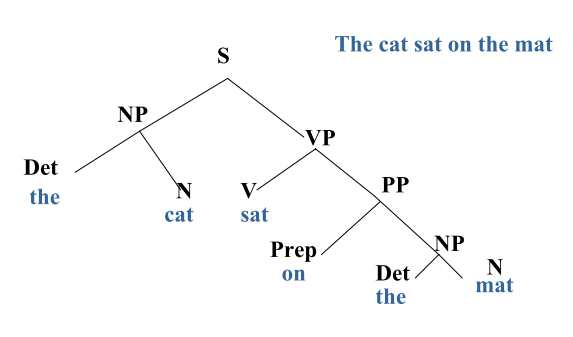
\includegraphics[width=0.7\linewidth,keepaspectratio]{nlproth3}
\end{center}



(Ref: The Role of Linguistics in  Natural Language Processing - 
Martha Palmer)
 \end{frame}
 
 
%%%%%%%%%%%%%%%%%%%%%%%%%%%%%%%%%%%%%%%%%%%%%%%%%%%%%%%%%%%%%%%%%%%%%%%%%%%%%%%%%%
\begin{frame}[fragile]
  \frametitle{Parses}
  \begin{center}
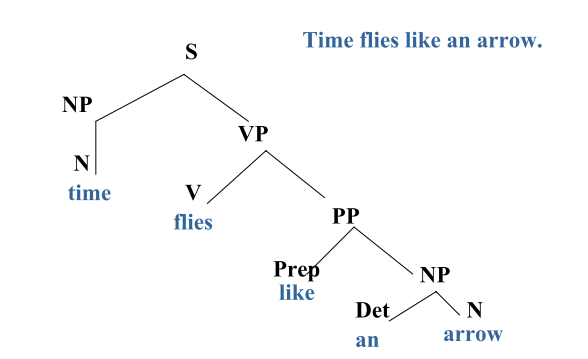
\includegraphics[width=0.7\linewidth,keepaspectratio]{nlproth4}
\end{center}



(Ref: The Role of Linguistics in  Natural Language Processing - 
Martha Palmer)
 \end{frame}
 
 %%%%%%%%%%%%%%%%%%%%%%%%%%%%%%%%%%%%%%%%%%%%%%%%%%%%%%%%%%%%%%%%%%%%%%%%%%%%%%%%%%
\begin{frame}[fragile]
  \frametitle{Parses}
  \begin{center}
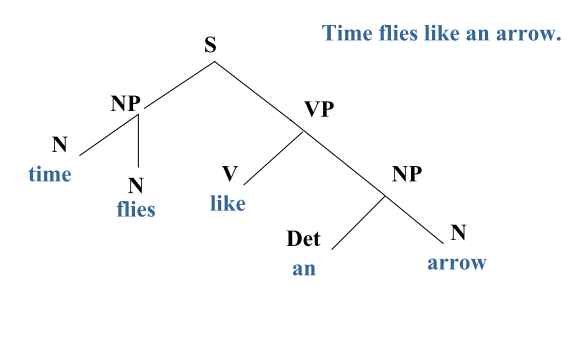
\includegraphics[width=0.7\linewidth,keepaspectratio]{nlproth5}
\end{center}



(Ref: The Role of Linguistics in  Natural Language Processing - 
Martha Palmer)
 \end{frame}
 
  %%%%%%%%%%%%%%%%%%%%%%%%%%%%%%%%%%%%%%%%%%%%%%%%%%%%%%%%%%%%%%%%%%%%%%%%%%%%%%%%%%
\begin{frame}[fragile]
  \frametitle{Simple Context Free Grammar in BNF 
notation}
  \begin{center}
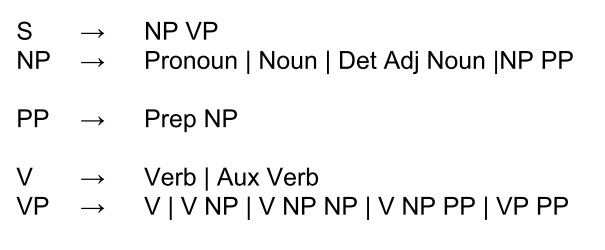
\includegraphics[width=0.7\linewidth,keepaspectratio]{nlproth6}
\end{center}



(Ref: The Role of Linguistics in  Natural Language Processing - 
Martha Palmer)
 \end{frame}
 
   %%%%%%%%%%%%%%%%%%%%%%%%%%%%%%%%%%%%%%%%%%%%%%%%%%%%%%%%%%%%%%%%%%%%%%%%%%%%%%%%%%
\begin{frame}[fragile]
  \frametitle{Top-down parse in progress}
Which rule worked?

Ex: [The, old, can, can, hold, the, water]

  \begin{center}
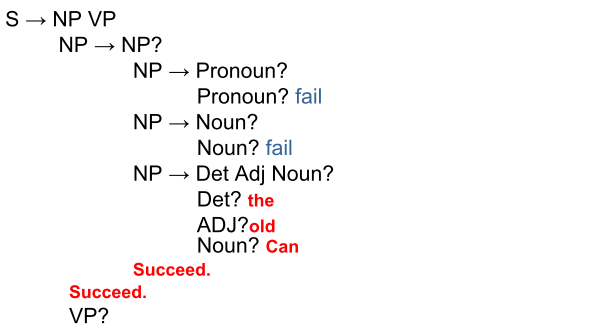
\includegraphics[width=0.7\linewidth,keepaspectratio]{nlproth7}
\end{center}

(Ref: The Role of Linguistics in  Natural Language Processing - 
Martha Palmer)
 \end{frame}
 
 
    %%%%%%%%%%%%%%%%%%%%%%%%%%%%%%%%%%%%%%%%%%%%%%%%%%%%%%%%%%%%%%%%%%%%%%%%%%%%%%%%%%
\begin{frame}[fragile]
  \frametitle{Top-down parse in progress}
Which rule worked?

Ex: [can, hold, the, water]

  \begin{center}
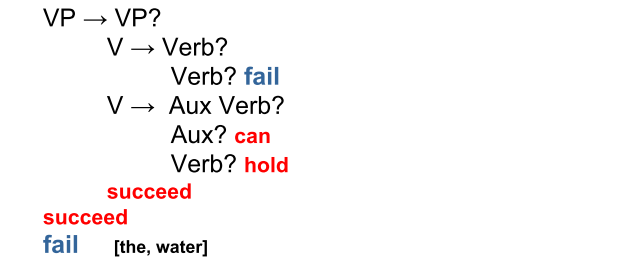
\includegraphics[width=0.7\linewidth,keepaspectratio]{nlproth8}
\end{center}

(Ref: The Role of Linguistics in  Natural Language Processing - 
Martha Palmer)
 \end{frame}
 
  
    %%%%%%%%%%%%%%%%%%%%%%%%%%%%%%%%%%%%%%%%%%%%%%%%%%%%%%%%%%%%%%%%%%%%%%%%%%%%%%%%%%
\begin{frame}[fragile]
  \frametitle{Top-down parse in progress}
Which rule worked?

Ex: [can, hold, the, water]

  \begin{center}
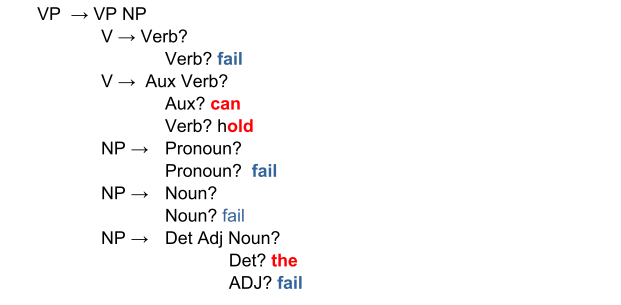
\includegraphics[width=0.7\linewidth,keepaspectratio]{nlproth9}
\end{center}

(Ref: The Role of Linguistics in  Natural Language Processing - 
Martha Palmer)
 \end{frame}
 
    %%%%%%%%%%%%%%%%%%%%%%%%%%%%%%%%%%%%%%%%%%%%%%%%%%%%%%%%%%%%%%%%%%%%%%%%%%%%%%%%%%
\begin{frame}[fragile]
  \frametitle{Top-down parse in progress}
Which rule worked?

Ex: [can, hold, the, water]

  \begin{center}
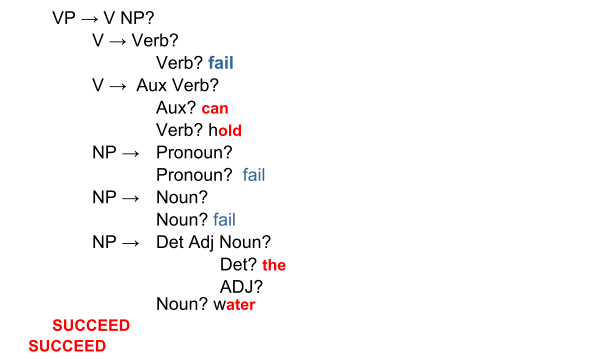
\includegraphics[width=0.7\linewidth,keepaspectratio]{nlproth10}
\end{center}

(Ref: The Role of Linguistics in  Natural Language Processing - 
Martha Palmer)
 \end{frame}
 
 
 
% %%%%%%%%%%%%%%%%%%%%%%%%%%%%%%%%%%%%%%%%%%%%%%%%%%%%%%%%%%%%%%%%%%%%%%%%%%%%%%%%%%
% \begin{frame}[fragile]
  % \frametitle{Phrase structure grammar}
  % \begin{center}
% 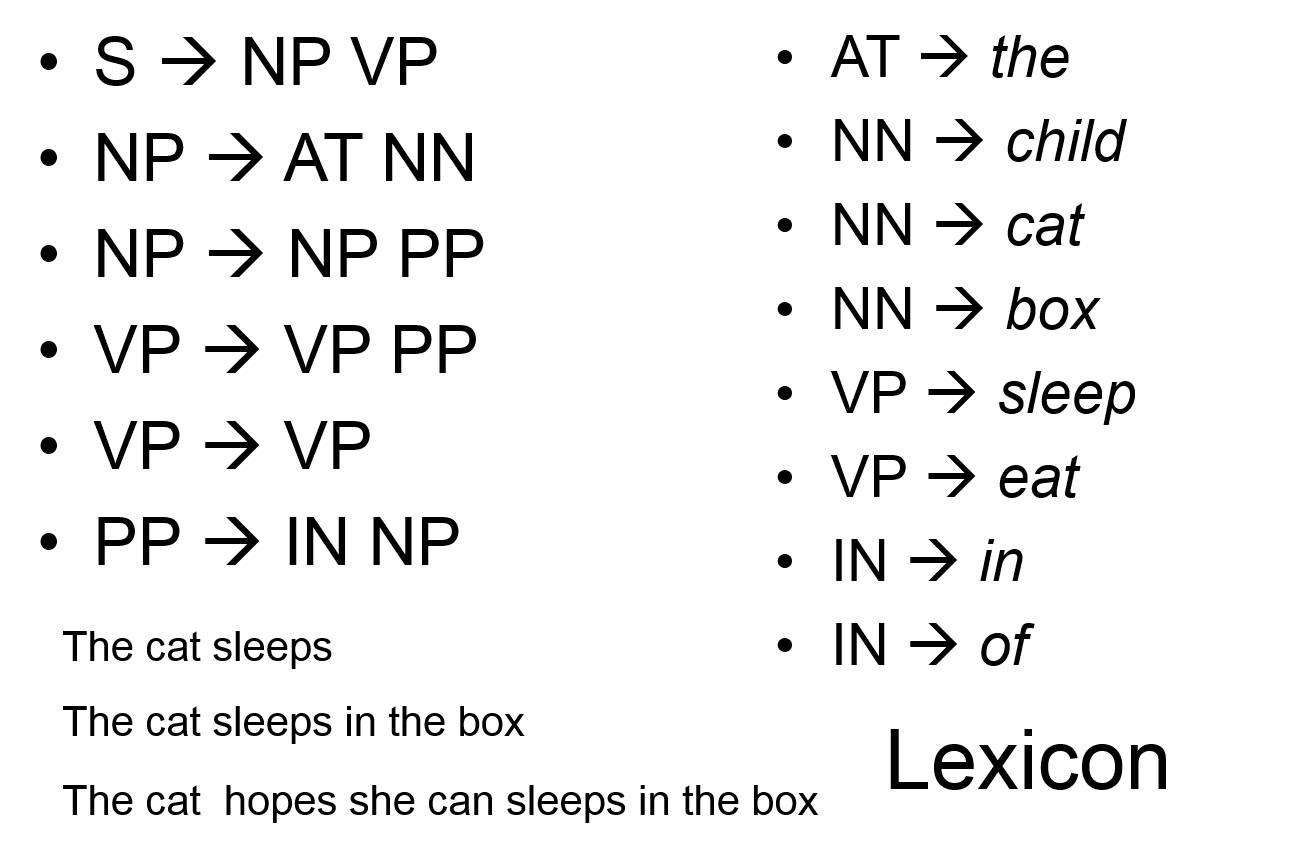
\includegraphics[width=\linewidth,keepaspectratio]{phase1}
% \end{center}
% \end{frame}

%%%%%%%%%%%%%%%%%%%%%%%%%%%%%%%%%%%%%%%%%%%%%%%%%%%%%%%%%%%%%%%%%%%%%%%%%%%%%%%%%%%
%\begin{frame}[fragile]
%  \frametitle{Context free grammars}
%  \begin{itemize}
%  \item The rewrite rules depend solely on the category and not on any surrounding context: Context Free Grammar
%  \item Main problems:
%
%    \begin{itemize}
%  \item Identify these grammars for natural languages (linguistics)
%  \item Known the grammar, identify the phrase structures of sentences (NLP, parsing)
%  \end{itemize}
%  \end{itemize}
%\end{frame}


%%%%%%%%%%%%%%%%%%%%%%%%%%%%%%%%%%%%%%%%%%%%%%%%%%%%%%%%%%%%%%%%%%%%%%%%%%%%%%%%%%
\begin{frame}[fragile]
  \frametitle{Phrase structure parsing}
  \begin{itemize}
  \item Parsing: the process of reconstructing the derivation(s) or phrase structure trees that give rise to a particular sequence of words
  \item Parse is a phrase structure tree:
``New art critics write reviews with computers''
  \begin{center}
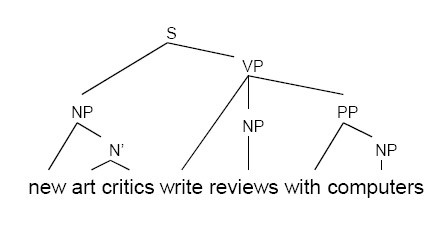
\includegraphics[width=0.7\linewidth,keepaspectratio]{phase2}
\end{center}
  \end{itemize}
\end{frame}

%%%%%%%%%%%%%%%%%%%%%%%%%%%%%%%%%%%%%%%%%%%%%%%%%%%%%%%%%%%%%%%%%%%%%%%%%%%%%%%%%%
\begin{frame}[fragile]
  \frametitle{Phrase structure parsing \& Ambiguity}
  \begin{itemize}
  \item PP Attachment Ambiguity
  \item  Why is it important for NLP?
``The children ate the cake with a spoon''
  \begin{center}
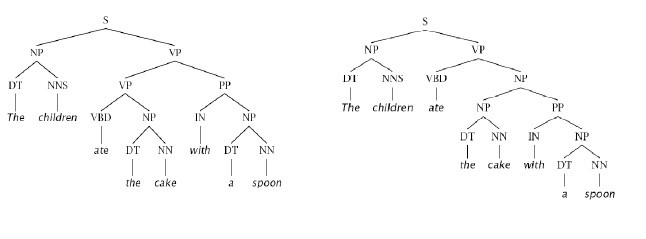
\includegraphics[width=\linewidth,keepaspectratio]{phase3}
\end{center}
  \end{itemize}
\end{frame}

%%%%%%%%%%%%%%%%%%%%%%%%%%%%%%%%%%%%%%%%%%%%%%%%%%%%%%%%%%%%%%%%%%%%%%%%%%%%%%%%%%
\begin{frame}[fragile]
  \frametitle{Phrase structure parsing \& Ambiguity}
  \begin{itemize}
  \item Both diagrams, first level: NP (The Children) + VP (ate the cake with a spoon)
  \item Diff in the second level for VP (ie right subtree)
  \item First diagram:  ate the cake + with a spoon
  \item Second diagram:  ate + the cake with a spoon (meaning the cake may have spoon embedded or drawn in it)
  \begin{center}
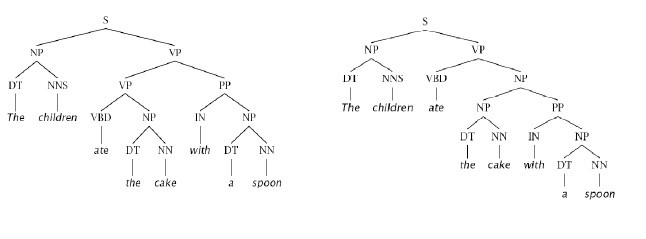
\includegraphics[width=\linewidth,keepaspectratio]{phase3}
\end{center}
  \end{itemize}
\end{frame}

% %%%%%%%%%%%%%%%%%%%%%%%%%%%%%%%%%%%%%%%%%%%%%%%%%%%%%%%%%%%%%%%%%%%%%%%%%%%%%%%%%%
% \begin{frame}[fragile]\frametitle{}

% \begin{center}
% {\Large Semnatics, in details}
% \end{center}
% \end{frame}


%%%%%%%%%%%%%%%%%%%%%%%%%%%%%%%%%%%%%%%%%%%%%%%%%%%%%%%%%%%%%%%%%%%%%%%%%%%%%%%%%%
\begin{frame}[fragile]
  \frametitle{Semantics}
 Semantics is the study of the meaning of words, construction and utterances
    \begin{itemize}
  \item Study of the meaning of individual words (lexical semantics)
  \item Study of how meanings of individual words are combined into the meaning of sentences (or larger units)
  \end{itemize}
\end{frame}


%%%%%%%%%%%%%%%%%%%%%%%%%%%%%%%%%%%%%%%%%%%%%%%%%%%%%%%%%%%%%%%%%%%%%%%%%%%%%%%%%%
\begin{frame}[fragile]\frametitle{Word Similarity}
 \begin{itemize}
 \item It's useful to know whether two words are similar
   \begin{itemize}
   \item Search: don't just find the exact terms you specify.
   \item Question Answering: handle synonyms.
   \item Parsing: what words act similarly to one another?
   \end{itemize}
 \item Different notions of \emph{similarity}:
 \item What words tend to co-occur?
 \item What words occur in similar contexts?
 \end{itemize}
\end{frame}

%%%%%%%%%%%%%%%%%%%%%%%%%%%%%%%%%%%%%%%%%%%%%%%%%%%%%%%%%%%%%%%%%%%%%%%%%%%%%%%%%%
\begin{frame}[fragile]
  \frametitle{Lexical semantics}
  How words are related with each other
  \begin{itemize}
  \item Hyponymy(child classes): scarlet, vermilion, carmine, and crimson are all hyponyms of red  
  \item Hypernymy (parent class): 
    \item Antonymy (opposite): Male, female
  \item Meronymy (part of): Tire is meromym of car
  \end{itemize}
    \begin{center}
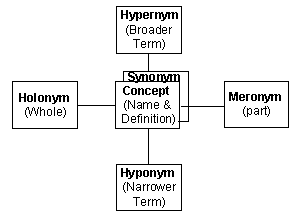
\includegraphics[width=0.5\linewidth,keepaspectratio]{hyp}
\end{center}
\end{frame}


%%%%%%%%%%%%%%%%%%%%%%%%%%%%%%%%%%%%%%%%%%%%%%%%%%%%%%%%%%%%%%%%%%%%%%%%%%%%%%%%%%
\begin{frame}[fragile]
 \frametitle{Semantics: beyond individual words}
 \begin{itemize}
 \item Once we have the meaning of the individual words, we need to assemble them to et the meaning of the whole sentence
 \item Hard because natural language does not obey the principle of compositionality by which the meaning of the whole can be predicted by the meanings of the parts, 
 \item E.g., the word white refers to different colors in the following expressions:  
     white paper; white hair; white skin; white wine

 \end{itemize}
\end{frame}

%%%%%%%%%%%%%%%%%%%%%%%%%%%%%%%%%%%%%%%%%%%%%%%%%%%%%%%%%%%%%%%%%%%%%%%%%%%%%%%%%%
\begin{frame}[fragile]
 \frametitle{Pragmatics}
 \begin{itemize}
 \item One of the important issues studied here is that of discourse analysis. 
A central problem there is that resolution of anaphoric relations.
An example:
Mary helped the other passenger out of the cab. The man had asked her to help him because of his foot injury. 

\item Anaphoric relations hold between Noun Phrases that refer to the same thing in the world. 
In the above example, there are quite a few ways to resolve the identify of "the man","him" and "his foot".
This issue is important in many applications, in particular in information extraction -- where there is a need to keep track of participants.
\item The Reference problem vs. the Co-reference problem.


 \end{itemize}
\end{frame}

%%%%%%%%%%%%%%%%%%%%%%%%%%%%%%%%%%%%%%%%%%%%%%%%%%%%%%%%%%%%%%%%%%%%%%%%%%%%%%%%%%
\begin{frame}[fragile]
 \frametitle{Summary}
 Linguistics is subdivided traditionally into 

 \begin{itemize}
 \item Phonetics (physical sounds of the language; consonants, vowels, intonation)
 \item Phonology (how sounds are mentally represented), 
 \item Morphology,
 \item Syntax, 
 \item Semantics and  
 \item Pragmatics.
 \item Most of the work within the statistics and learning-based approaches to natural language is done in the areas of Syntax, Semantics, and some Pragmatics and this will be our main concern in this course as well. 
 \item Phonetics is also studied using related methods, within the Speech community, and the techniques we will present in this course could be used there, as well as in Morphology and Discourse analysis.
 \end{itemize}
\end{frame}



%%%%%%%%%%%%%%%%%%%%%%%%%%%%%%%%%%%%%%%%%%%%%%%%%%%%%%%%%%%%%%%%%%%%%%%%%%%%%%%%%%%
%\begin{frame}[fragile]
%  \frametitle{Introduction}
%  \begin{itemize}
%  \item language resources, types, proliferation
%  \item role in NLP, CL
%  \item enablers: storage/XML/Unicode; digital publication; resource catalogues
%  \item obstacles: discovery, access, format, tool
%  \item data types: texts and lexicons
%  \item useful ways to access data using Python: csv, html, xml
%  \item adding a corpus to NLTK
%  \end{itemize}
%\end{frame}
%
%%%%%%%%%%%%%%%%%%%%%%%%%%%%%%%%%%%%%%%%%%%%%%%%%%%%%%%%%%%%%%%%%%%%%%%%%%%%%%%%%%%
%\begin{frame}[fragile]\frametitle{Linguistic Databases}
%\begin{itemize}
%\item Field linguistics
%\item Corpora
%\item Reference Corpus
%\end{itemize}
%\end{frame}
%
%
%%%%%%%%%%%%%%%%%%%%%%%%%%%%%%%%%%%%%%%%%%%%%%%%%%%%%%%%%%%%%%%%%%%%%%%%%%%%%%%%%%%
%\begin{frame}[fragile]\frametitle{Lifecycle}
%
%\begin{itemize}
%\item Create
%\item Annotate texts
%\item Refine lexicon
%\item Organize structure
%\item Publish
%\end{itemize}
%\end{frame}
%
%%%%%%%%%%%%%%%%%%%%%%%%%%%%%%%%%%%%%%%%%%%%%%%%%%%%%%%%%%%%%%%%%%%%%%%%%%%%%%%%%%%%
%\begin{frame}[fragile]
%\frametitle{Evolution}
%\begin{center}
%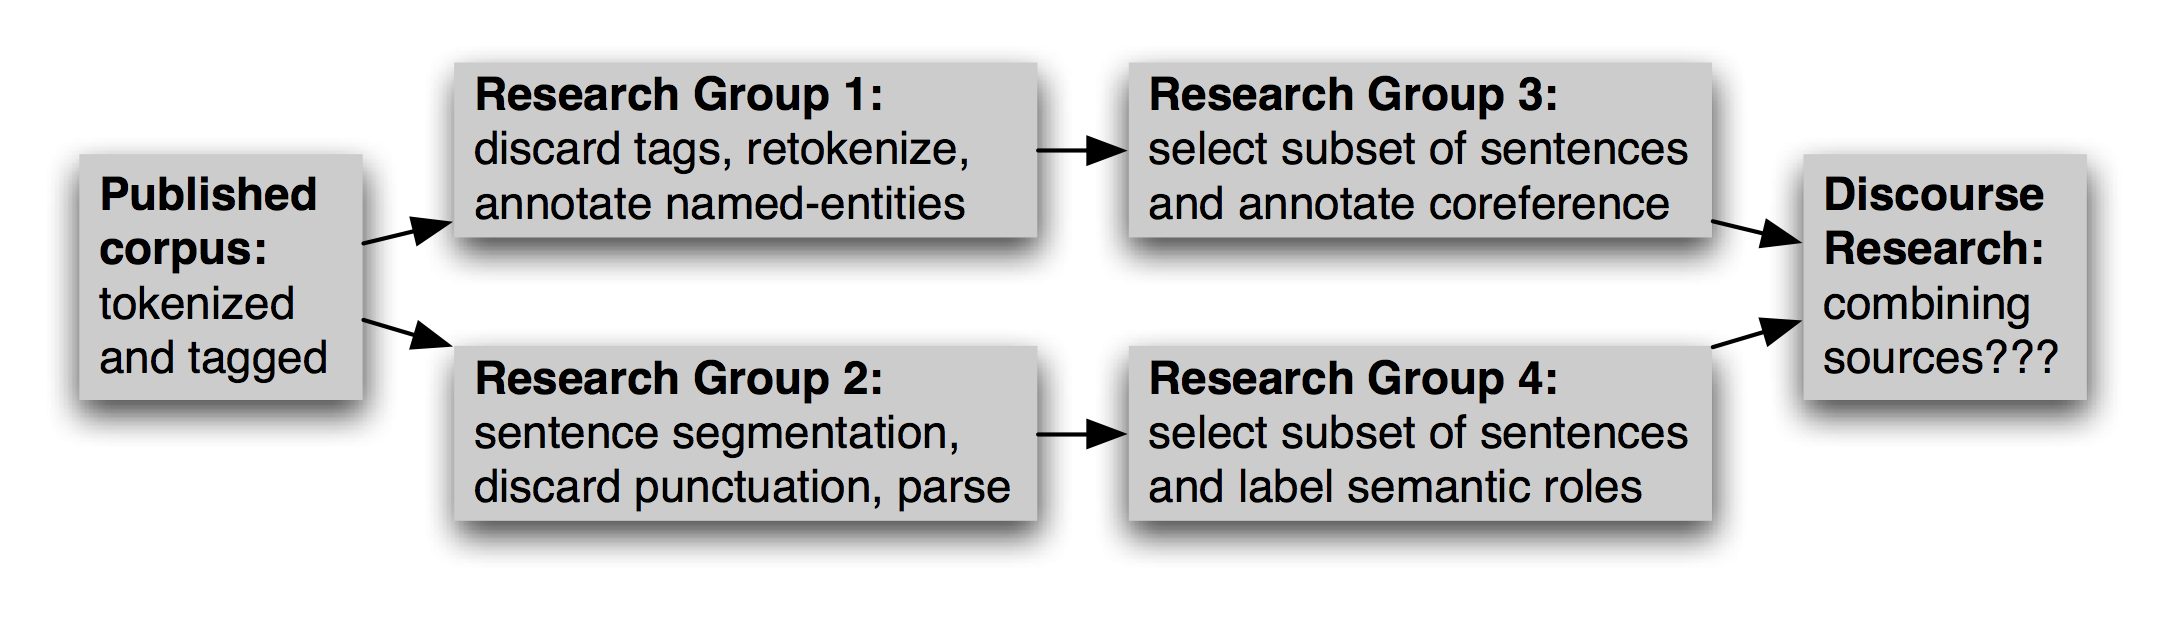
\includegraphics[width=\linewidth,keepaspectratio]{evolution}
%\end{center}
%\end{frame}
%
%
%%%%%%%%%%%%%%%%%%%%%%%%%%%%%%%%%%%%%%%%%%%%%%%%%%%%%%%%%%%%%%%%%%%%%%%%%%%%%%%%%%%
%\begin{frame}[fragile]
%\frametitle{Creating Data: Primary Data}
%
%\begin{itemize}
%\item Spiders
%\item Recording
%\item Texts
%\end{itemize}
%\end{frame}
%
%%%%%%%%%%%%%%%%%%%%%%%%%%%%%%%%%%%%%%%%%%%%%%%%%%%%%%%%%%%%%%%%%%%%%%%%%%%%%%%%%%%
%\begin{frame}[fragile]\frametitle{Creating Data: Annotation}
%\begin{itemize}
%\item Linguistic annotation
%\item Tools: \verb|http://www.exmaralda.org/annotation/|
%\end{itemize}
%\end{frame}
%
%%%%%%%%%%%%%%%%%%%%%%%%%%%%%%%%%%%%%%%%%%%%%%%%%%%%%%%%%%%%%%%%%%%%%%%%%%%%%%%%%%%%
%%\pgfdeclareimage[width=\textwidth]{windowdiff}{windowdiff}
%%\begin{frame}[fragile]\frametitle{Creating Data: Inter-Annotator Agreement}
%%  \begin{itemize}
%%  \item Kappa statistic
%%  \item Windowdiff
%%  \end{itemize}
%%  \begin{center}
%%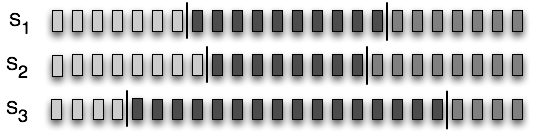
\includegraphics[width=\linewidth,keepaspectratio]{windowdiff}
%%\end{center}
%%\end{frame}
%%
%%%%%%%%%%%%%%%%%%%%%%%%%%%%%%%%%%%%%%%%%%%%%%%%%%%%%%%%%%%%%%%%%%%%%%%%%%%%%%%%%%%%
%%\begin{frame}[fragile]\frametitle{Processing Toolbox Data}
%%
%%\begin{itemize}
%%\item single most popular tool for managing linguistic field data
%%\item many kinds of validation and formatting not supported by Toolbox software
%%\item each file is a collection of \textit{entries} (aka
%%  \textit{records})
%%\item each entry is made up of one or more \textit{fields}
%%\item we can apply our programming methods, including chunking and parsing
%%\end{itemize}
%%\end{frame}
%%
%%%%%%%%%%%%%%%%%%%%%%%%%%%%%%%%%%%%%%%%%%%%%%%%%%%%%%%%%%%%%%%%%%%%%%%%%%%%%%%%%%%%
%%\begin{frame}[fragile]\frametitle{Toolbox Example}
%%\small
%%
%%\begin{lstlisting}
%%\lx kaa
%%\ps N.M
%%\cl isi
%%\ge cooking banana
%%\gp banana bilong kukim
%%\sf FLORA
%%\dt 12/Feb/2005
%%\ex Taeavi iria kaa isi kovopaueva kaparapasia.
%%\xp Taeavi i bin planim gaden banana bilong kukim tasol long paia.
%%\xe Taeavi planted banana in order to cook it.
%%\end{lstlisting}
%%\end{frame}
%
%%%%%%%%%%%%%%%%%%%%%%%%%%%%%%%%%%%%%%%%%%%%%%%%%%%%%%%%%%%%%%%%%%%%%%%%%%%%%%%%%%%
%\begin{frame}[fragile]\frametitle{Adding a Corpus to NLTK}
%
%\begin{itemize}
%\item Corpus path
%\item Corpus readers
%\end{itemize}
%\end{frame}
%
%
%%%%%%%%%%%%%%%%%%%%%%%%%%%%%%%%%%%%%%%%%%%%%%%%%%%%%%%%%%%%%%%%%%%%%%%%%%%%%%%%%%%%
%%\begin{frame}[fragile]\frametitle{Publishing}
%%
%%\begin{itemize}
%%\item metadata: DC, OLAC
%%\item repositories
%%\item search
%%\item demo
%%\end{itemize}
%%
%%\end{frame}
%
